\begin{center}
  \textsf{Листок 5.}
\end{center}
\vspace{0.01mm}
\nopagebreak[2]
\task{Автомобиль с работающим двигателем въезжает на обледенелую
  гору, поверхность которой образует угол $\alpha$ с горизонтом. Какой
  высоты гору может преодолеть автомобиль, если его начальная скорость
  при въезде на неё равна $V$, а коэффициент трения колёс о лёд $k$?}

\task{Каков радиус орбиты спутника, лежащей в экваториальной
  плоскости, если тот всё время находится в зените над одной и той же
  точкой земной поверхности?  }

\taskpic{ Найдите ускорение грузов, если масса каждого груза равна
  $m$. Массами нитей и блоков пренебречь, нити нерастяжимы, трение
  отсутствует.
}{
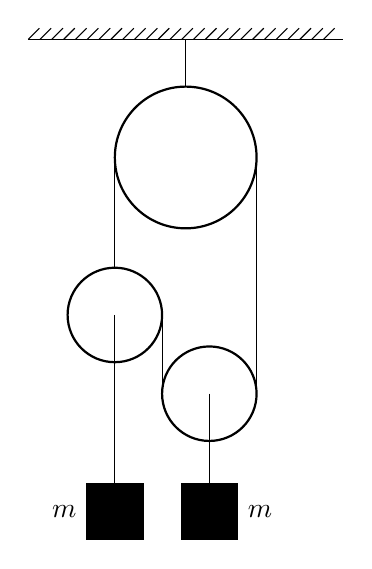
\begin{tikzpicture}[interface/.style={postaction={draw,decorate,decoration={border,angle=45,amplitude=0.2cm,segment length=1.5mm}}},>=latex]
  \draw[interface] (1,0) -- (5,0);
  \draw (3,0) -- (3,-1.5);
  \filldraw[thick,white,draw=black] (3,-1.5) circle (0.9);
  \draw (2.1,-1.5) -- ++(0,-2) (3.9,-1.5) -- ++(0,-3);
  \filldraw[thick,white,draw=black] (2.1,-3.5) circle (0.6);
  \filldraw[thick,white,draw=black] (3.3,-4.5) circle (0.6);
  \draw (2.7,-3.5) -- +(0,-1);
  \draw (2.1,-3.5) -- +(0,-2.5);
  \draw (3.3,-4.5) -- +(0,-1.5);
  \node [rectangle,fill=black,draw=black,thick,label={left:$m$},minimum
  height=0.7cm,minimum width=0.7cm] at (2.1,-6) {};
  \node
  [rectangle,fill=black,draw=black,thick,label={right:$m$},minimum
  height=0.7cm,minimum width=0.7cm] at (3.3,-6) {};
\end{tikzpicture}
}

\task{Лестница опирается на вертикальную стену и пол. При каких
  значениях угла между лестницей и полом она может стоять, если
  коэффициент трения лестницы о пол и о стену равен $k_1$ и $k_2$
  соответственно?}

%%% Local Variables: 
%%% mode: latex
%%% TeX-master: "../../../report"
%%% End: 
